% !TEX root = ../main.tex
\clearpage
\section{Additional ablations}
\label{app:additionalablations}

\subsection{SCCFG sensitivity}
\label{app:sccfgsweep}
We sweep SCCFG coefficients $\{1,2,3,4\}$ at the epoch-21 ELF-L checkpoints on GSM8K and MATH500. Both use ELF/prompt EMA $.9999/.9999$, async $(2.5,2,1.5)$, 32 denoising steps, CFG 1, and seeds 42/123. The coefficient is applied during both denoising and terminal decoding; SCCFG 1 retains recurrent self-conditioning. Separate seeded invocations match the initial noise across coefficients.

\begin{figure}[htbp]
\centering
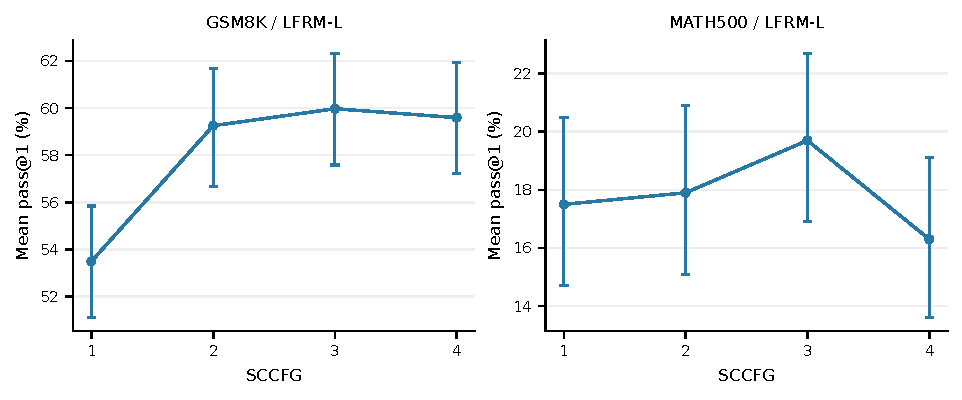
\includegraphics[width=\linewidth]{figures/sccfg_sweep.pdf}
\caption{SCCFG sensitivity on full GSM8K and MATH500 test sets at ELF-L epoch 21. Points average seeds 42/123; bars show pointwise 95\% problem-bootstrap intervals for absolute pass@1. Checkpoints and other inference settings are fixed. Table~\ref{tab:sccfgsweepvalues} reports the individual seeds, means, across-seed SDs, and paired differences. This is a test-set sensitivity analysis.}
\label{fig:sccfgsweep}
\end{figure}

% !TEX root = ../main.tex
\begin{table}[htbp]
\caption{Numerical values for Figure~\ref{fig:sccfgsweep}. Pass@1 reports mean accuracy with across-seed SD in parentheses; individual seeds are also shown. Differences from SCCFG 2 have paired 95\% problem-bootstrap intervals. Accuracy and differences are in percentage points.}
\label{tab:sccfgsweepvalues}
\centering\small
\setlength{\tabcolsep}{4pt}
\begin{tabular}{@{}lrrrrl@{}}
\toprule
Dataset / SCCFG & Seed 42 & Seed 123 & Pass@1 (SD) & Pass@2 & $\Delta$ vs.\ 2 [95\% CI] \\
\midrule
GSM8K / 1 & 53.37 & 53.60 & 53.49 {\scriptsize (0.16)} & 64.22 & $-5.76$ $[-7.13, -4.36]$ \\
GSM8K / 2 & 59.36 & 59.14 & 59.25 {\scriptsize (0.16)} & 68.31 & --- \\
GSM8K / 3 & 59.59 & 60.35 & 59.97 {\scriptsize (0.54)} & 69.52 & $+0.72$ $[-0.49, 1.93]$ \\
GSM8K / 4 & 59.36 & 59.82 & 59.59 {\scriptsize (0.32)} & 67.85 & $+0.34$ $[-1.02, 1.74]$ \\
\midrule
MATH500 / 1 & 16.20 & 18.80 & 17.50 {\scriptsize (1.84)} & 26.20 & $-0.40$ $[-2.50, 1.70]$ \\
MATH500 / 2 & 17.00 & 18.80 & 17.90 {\scriptsize (1.27)} & 26.40 & --- \\
MATH500 / 3 & 19.40 & 20.00 & 19.70 {\scriptsize (0.42)} & 29.60 & $+1.80$ $[-0.20, 3.80]$ \\
MATH500 / 4 & 16.40 & 16.20 & 16.30 {\scriptsize (0.14)} & 24.80 & $-1.60$ $[-3.80, 0.50]$ \\
\bottomrule
\end{tabular}
\end{table}


In this initial two-seed sweep, SCCFG 3 gives the highest observed mean on both tasks: 59.97\% on GSM8K and 19.70\% on MATH500, compared with 59.25\% and 17.90\% at SCCFG 2. The paired gains over 2 are $+0.72$ points ($[-0.49,1.93]$) and $+1.80$ ($[-0.20,3.80]$), respectively; both intervals include zero. On GSM8K, SCCFG 2 improves over SCCFG 1 by 5.76 points ($[4.36,7.13]$), supporting the value of retaining guidance in this model. MATH500 has a different sensitivity profile: its SCCFG-2-minus-1 difference is only 0.40 points, with an interval including zero. The sweep motivates preserving SCCFG during NFT but does not isolate the benefit of our particular NFT guidance correction.

\subsection{Expanded MATH500 comparison}
\label{app:mathsccfg3}
We subsequently compare SCCFG 3 against 2 on MATH500 at both epoch 21 and NFT update 600, matching checkpoints, prompts, scoring, arithmetic, and ordered seed lists. At 8, 16, 32, and 64 denoising steps, each checkpoint has 64, 32, 16, and 8 draws per problem, respectively. The coefficient changes during both denoising and terminal decoding; all other settings, including ELF/prompt EMA $.9999/.9999$ before NFT and $.99/.99$ afterward, remain fixed. Math-Verify is the primary scorer. This follow-up measures sensitivity on the same test benchmark; it is not an independent development-set selection of guidance.

% !TEX root = ../main.tex
\begin{table}[htbp]
\caption{MATH500 pass@1 sensitivity to SCCFG at matched checkpoints and generation seeds. Entries are mean accuracy percentages with across-seed SDs in parentheses. Differences are SCCFG 3 minus 2 in percentage points, with paired 95\% problem-bootstrap intervals. Each NFE uses the complete draw cohort.}
\label{tab:mathsccfg3}
\centering\small
\setlength{\tabcolsep}{5pt}
\begin{tabular}{@{}lrrrrl@{}}
\toprule
Checkpoint & NFE & Draws & SCCFG 2 (SD) & SCCFG 3 (SD) & Difference [95\% CI] \\
\midrule
Pre-NFT & 8 & 64 & 13.88 {\scriptsize (1.19)} & 15.23 {\scriptsize (1.16)} & $+1.34$ $[0.97, 1.73]$ \\
Pre-NFT & 16 & 32 & 16.39 {\scriptsize (1.20)} & 17.93 {\scriptsize (1.30)} & $+1.53$ $[1.07, 2.01]$ \\
Pre-NFT & 32 & 16 & 17.89 {\scriptsize (1.31)} & 19.65 {\scriptsize (1.37)} & $+1.76$ $[0.99, 2.56]$ \\
Pre-NFT & 64 & 8 & 18.85 {\scriptsize (1.38)} & 21.18 {\scriptsize (0.70)} & $+2.33$ $[1.27, 3.43]$ \\
\midrule
NFT 600 & 8 & 64 & 16.31 {\scriptsize (1.36)} & 17.45 {\scriptsize (1.33)} & $+1.14$ $[0.76, 1.53]$ \\
NFT 600 & 16 & 32 & 20.09 {\scriptsize (1.23)} & 20.93 {\scriptsize (1.26)} & $+0.84$ $[0.31, 1.39]$ \\
NFT 600 & 32 & 16 & 22.08 {\scriptsize (1.41)} & 22.60 {\scriptsize (1.58)} & $+0.53$ $[-0.19, 1.29]$ \\
NFT 600 & 64 & 8 & 23.60 {\scriptsize (1.79)} & 24.68 {\scriptsize (1.27)} & $+1.08$ $[0.00, 2.20]$ \\
\bottomrule
\end{tabular}
\end{table}


SCCFG 3 raises mean pass@1 at every tested depth for both checkpoints, with the clearest evidence before NFT. At the retained 64-step headline budget, the supervised model improves by $2.33$ points ($[1.27,3.43]$), and the NFT model by $1.08$ ($[0.00,2.20]$). Holding SCCFG at 3, NFT still improves pass@1 over the supervised model by $3.50$ points ($[2.28,4.75]$). These results motivate the SCCFG 3 MATH500 headline rows in Tables~\ref{tab:headlinecomparison}--\ref{tab:headlinelownfe}. GSM8K retains SCCFG 2, as do all curves in Figure~\ref{fig:headlinestages}.

The pass@1 improvement does not imply a uniform improvement in multi-sample coverage. For the NFT checkpoint at 32 steps and 16 draws, changing SCCFG from 2 to 3 reduces oracle accuracy from 60.40\% to 56.80\% ($-3.60$ points; $[-6.41,-0.80]$), while voting changes by only $+0.04$ points ($[-1.93,2.14]$). At 64 steps and eight draws, post-NFT voting increases from 32.42\% to 33.38\%, but the paired gain of $0.96$ points has interval $[-1.60,3.48]$. Like the NFT comparisons, the guidance sweep illustrates why single-sample quality, oracle coverage, and answer selection should be reported separately. All intervals here use 4,000 paired problem-bootstrap replicates with seed 20260918, conditional on the fixed checkpoints and draws, without multiple-comparison adjustment.
